% Beamer presentation: from Bayesian optimization to an agentic, Claude-driven
% tuning loop for a Skipper-CCD read out by an LTA.
%
% Build:  cd docs/presentation && pdflatex skipperopt_agents.tex   (run twice)
% Optional figure: copy a convergence plot from a run to
%   figures/convergence.pdf   (e.g. images/skipper/ai/<date>/results-skipper.pdf)
% Lines marked  %% FILL IN  need numbers from your own runs / the Console.

\documentclass[aspectratio=169,10pt]{beamer}

\usetheme{default}
\usecolortheme{default}
\setbeamertemplate{navigation symbols}{}
\setbeamertemplate{footline}[frame number]
\definecolor{accent}{RGB}{31,94,140}
\definecolor{warm}{RGB}{190,90,40}
\definecolor{soft}{RGB}{235,240,245}
\setbeamercolor{frametitle}{fg=accent}
\setbeamercolor{title}{fg=accent}
\setbeamercolor{structure}{fg=accent}
\setbeamercolor{block title}{bg=accent,fg=white}
\setbeamercolor{block body}{bg=soft}
\setbeamerfont{frametitle}{series=\bfseries}

\usepackage[T1]{fontenc}
\usepackage{lmodern}
\usepackage{booktabs}
\usepackage{tikz}
\usetikzlibrary{arrows.meta,positioning,shapes.geometric,fit,backgrounds}
\usepackage{listings}
\lstset{basicstyle=\ttfamily\scriptsize,columns=fullflexible,keepspaces=true,
        frame=single,rulecolor=\color{gray!40},backgroundcolor=\color{soft},
        showstringspaces=false,breaklines=true}

\newcommand{\fillin}[1]{\textcolor{warm}{\textbf{[#1]}}}

\tikzset{
  box/.style={draw=accent,thick,rounded corners=3pt,fill=soft,align=center,
              minimum height=9mm,inner sep=4pt,font=\small},
  agent/.style={box,fill=accent!12,minimum width=30mm},
  hw/.style={box,draw=warm,fill=warm!10},
  arr/.style={-{Stealth[length=2.2mm]},thick,draw=accent},
  lbl/.style={font=\scriptsize,text=black!70,align=center},
}

\title{From Bayesian Optimization to an Agentic, Claude-Driven Tuning Loop}
\subtitle{Skipper-CCD operating-point optimization with an LTA readout}
\author{Juan Cruz Estrada Vigil}
\institute{}   %% FILL IN institution
\date{\today}

\begin{document}

% ---------------------------------------------------------------------------
\begin{frame}
  \titlepage
\end{frame}

% ---------------------------------------------------------------------------
\begin{frame}{Outline}
  \begin{enumerate}
    \item The starting point: Bayesian optimization of a Skipper-CCD
    \item Code review: what to watch for
    \item Agentic version: three cooperating agents
    \item Claude as the optimizer
    \item Running it in the lab: what went wrong and how it was fixed
    \item Cost
    \item Lab notebook: memory across campaigns
    \item GP vs.\ Claude, open questions, next steps
  \end{enumerate}
\end{frame}

% ===========================================================================
\section{Starting point}
% ===========================================================================

\begin{frame}{The problem}
  \begin{columns}[T]
    \begin{column}{0.52\textwidth}
      \begin{itemize}
        \item Skipper-CCD read out with an \textbf{LTA} controller
        \item Find the operating parameters that give the best images
        \item Each evaluation is a \textbf{real measurement}:
              expose (LED) $\rightarrow$ set parameters $\rightarrow$ read out
              $\rightarrow$ score
        \item Expensive, noisy, black-box $\Rightarrow$ Bayesian optimization
      \end{itemize}
    \end{column}
    \begin{column}{0.44\textwidth}
      \centering\small
      \begin{tabular}{lrl}
        \toprule
        Parameter & Range & \\
        \midrule
        $V_{dd}$         & $[-23,-10]$ & V \\
        $V_{drain}$      & $[-23,-10]$ & V \\
        $V_{r}$          & $[-8,-5]$   & V \\
        \texttt{delay\_H\_overlap} & $[10,30]$ & clk \\
        \bottomrule
      \end{tabular}

      \vspace{2mm}
      {\scriptsize Optimizer works in $[-1,1]^4$; values mapped to physical units.}
    \end{column}
  \end{columns}
\end{frame}

\begin{frame}{The objective function}
  From each image: active region and overscan region
  \[
    \text{gain} = \operatorname{median}(\text{active}) - \operatorname{median}(\text{overscan}),
    \qquad
    \sigma_{os} = \operatorname{std}(\text{overscan})
  \]
  \[
    F = \min\!\left(\left|\frac{\sigma_{os}}{\text{gain}}\right|,\ 1000\right)
        \;+\; \sum_i c_i\,\text{penalty}_i^{\,p_i}
    \qquad\text{(lower is better)}
  \]
  \begin{itemize}
    \item With a fixed LED exposure, gain $\propto$ ADU/e$^-$, so $F$ tracks the
          read noise in electrons
    \item Optional penalties (negative gain, saturation, \dots) are configurable;
          all off in the current campaign
  \end{itemize}
\end{frame}

\begin{frame}{The original loop}
  \centering
  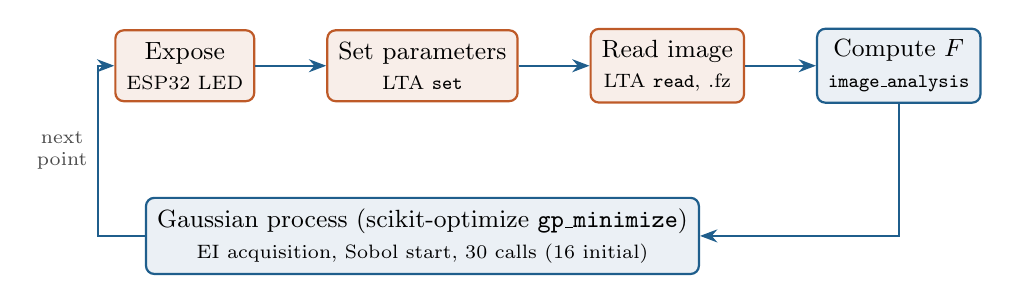
\begin{tikzpicture}[node distance=7mm and 9mm]
    \node[hw] (exp) {Expose\\\scriptsize ESP32 LED};
    \node[hw,right=of exp] (set) {Set parameters\\\scriptsize LTA \texttt{set}};
    \node[hw,right=of set] (read) {Read image\\\scriptsize LTA \texttt{read}, .fz};
    \node[box,right=of read] (f) {Compute $F$\\\scriptsize \texttt{image\_analysis}};
    \node[box,below=12mm of set,minimum width=60mm] (gp)
      {Gaussian process (scikit-optimize \texttt{gp\_minimize})\\
       \scriptsize EI acquisition, Sobol start, 30 calls (16 initial)};
    \draw[arr] (exp) -- (set);
    \draw[arr] (set) -- (read);
    \draw[arr] (read) -- (f);
    \draw[arr] (f) |- (gp);
    \draw[arr] (gp.west) -- ++(-6mm,0) |- node[lbl,pos=0.25,left]{next\\point} (exp.west);
  \end{tikzpicture}

  \vspace{4mm}
  \begin{itemize}\small
    \item Modular: \texttt{lta\_control} (hardware), \texttt{image\_analysis}
          (FITS + $F$), \texttt{bo\_core} (optimizer, CSV, plots)
    \item One JSON config per campaign; warm restart from a previous run
  \end{itemize}
\end{frame}

% ===========================================================================
\section{Review}
% ===========================================================================

\begin{frame}{Code review: things to watch}
  \begin{itemize}
    \item \textbf{Stale images}: shell return codes ignored and the newest
          \texttt{.fz} is scored, so a failed readout would be scored using
          the previous image
    \item \textbf{Bad amplifier states can score well}: \texttt{abs()} hides
          an inverted gain; a clipped output has $\sigma_{os}\to 0$
    \item \textbf{Real example} from a lab run:
          \begin{center}\small
          \begin{tabular}{cccc|ccc}
            $V_{dd}$ & $V_{drain}$ & $V_r$ & delay & $\sigma_{os}$ & gain & $F$\\\midrule
            $-10.3$ & $-12.5$ & $-5.2$ & 15 & 31924 & $-3544$ & 9.0
          \end{tabular}\end{center}
          a broken output still gets a finite, ``reasonable'' score
    \item \textbf{No settling time} after changing bias voltages
    \item \textbf{Noisy $F$}: the best \emph{measured} point may be a lucky draw
    \item \textbf{Resume file} only written at the end of a run
  \end{itemize}
  \vspace{1mm}
  {\scriptsize Kept as-is on purpose (no functional changes); the resume issue was fixed later.}
\end{frame}

% ===========================================================================
\section{Agentic version}
% ===========================================================================

\begin{frame}{Step 1: three cooperating agents}
  \centering
  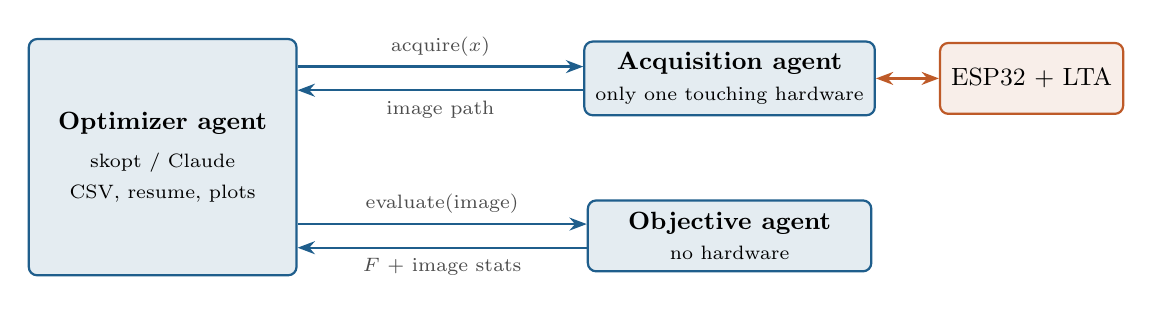
\begin{tikzpicture}
    \node[agent,minimum height=30mm,minimum width=34mm] (opt) at (0,0)
      {\textbf{Optimizer agent}\\[1mm]\scriptsize skopt / Claude\\\scriptsize CSV, resume, plots};
    \node[agent,minimum width=36mm] (acq) at (7.2,1.0)
      {\textbf{Acquisition agent}\\\scriptsize only one touching hardware};
    \node[agent,minimum width=36mm] (obj) at (7.2,-1.0)
      {\textbf{Objective agent}\\\scriptsize no hardware};
    \node[hw,right=8mm of acq] (hwn) {ESP32 + LTA};
    \coordinate (a1) at (0,1.15);  \coordinate (a2) at (0,0.85);
    \coordinate (b1) at (0,-0.85); \coordinate (b2) at (0,-1.15);
    \draw[arr] (opt.east |- a1) -- node[lbl,above]{acquire($x$)} (acq.west |- a1);
    \draw[arr] (acq.west |- a2) -- node[lbl,below]{image path} (opt.east |- a2);
    \draw[arr] (opt.east |- b1) -- node[lbl,above]{evaluate(image)} (obj.west |- b1);
    \draw[arr] (obj.west |- b2) -- node[lbl,below]{$F$ + image stats} (opt.east |- b2);
    \draw[{Stealth[length=2.2mm]}-{Stealth[length=2.2mm]},thick,draw=warm] (acq) -- (hwn);
  \end{tikzpicture}

  \vspace{3mm}
  \begin{itemize}\small
    \item Each agent is its own process (Python \texttt{multiprocessing}, standard library only)
    \item Messages are plain JSON dicts: ready for sockets or an LLM later
    \item Every message is logged to \texttt{<run>\_messages.jsonl}
    \item Same command line, same config, same output files
  \end{itemize}
\end{frame}

\begin{frame}[fragile]{Messages between agents}
\begin{lstlisting}
{"id": 7, "kind": "acquire", "sender": "optimizer",
 "payload": {"iteration": 3, "x_norm": [0.12, -0.40, 0.75, -0.05]}}

{"id": 8, "kind": "reply", "sender": "acquisition", "reply_to": 7, "ok": true,
 "payload": {"image_path": ".../optimize_76.fz"}}

{"id": 9, "kind": "evaluate", "sender": "optimizer",
 "payload": {"iteration": 3, "image_path": ".../optimize_76.fz"}}

{"id": 10, "kind": "reply", "sender": "objective", "reply_to": 9, "ok": true,
 "payload": {"F": 0.0296, "stats": {"noise_overscan": 636.4,
             "charge_overscan": 5310.0, "charge_active": 26812.5, "gain": 21502.5}}}
\end{lstlisting}
  \small
  \begin{itemize}
    \item An agent error comes back as \texttt{"ok": false} with its traceback;
          the run stops cleanly and the other agents are shut down
  \end{itemize}
\end{frame}

\begin{frame}{Validation: same results as the original}
  \begin{columns}[T]
    \begin{column}{0.55\textwidth}
      Simulated hardware for testing:
      \begin{itemize}\small
        \item fake \texttt{lta.sh}: synthetic images whose noise and signal
              depend on the voltages set
        \item fake ESP32 and FITS reader
      \end{itemize}
      Both drivers, same config and seed:
      \begin{itemize}\small
        \item identical \texttt{gp\_results.csv}, progress CSV and image files
        \item identical results on warm restart
        \item agent failure $\rightarrow$ clean stop with the agent's error
      \end{itemize}
    \end{column}
    \begin{column}{0.42\textwidth}
      \begin{block}{Test suite}
        \small
        17 automated tests, all passing\\[1mm]
        equivalence, message log, resume, failures,
        Claude optimizer (with a fake Claude), retries, cost, notebook
      \end{block}
      \vspace{2mm}
      {\scriptsize Runs without hardware, network or API key:\\
       \texttt{python -m pytest tests}}
    \end{column}
  \end{columns}
\end{frame}

\begin{frame}{First lab deployment: one surprise}
  \begin{itemize}
    \item Error: \emph{``No .fz image found''}, but the LTA said \emph{``Read done''}
    \item Cause: relative output path \texttt{images/...}
      \begin{itemize}\small
        \item Python resolved it from \emph{its} working directory
        \item the LTA daemon resolved it from \emph{its own} directory
        \item $\Rightarrow$ images written to one folder, searched for in another
      \end{itemize}
    \item Fix: absolute \texttt{output\_base} in the config (no code change)
    \item Not specific to agents: the original script had the same latent issue
  \end{itemize}
\end{frame}

% ===========================================================================
\section{Claude as optimizer}
% ===========================================================================

\begin{frame}[fragile]{Step 2: Claude replaces the Gaussian process}
  \begin{columns}[T]
    \begin{column}{0.52\textwidth}
      \begin{enumerate}\small
        \item \textbf{Sobol start}: 8 space-filling points (as for the GP)
        \item \textbf{Each further point}: Claude gets
          \begin{itemize}\scriptsize
            \item parameter descriptions and bounds, objective definition
            \item \emph{all} measurements so far, in physical units
            \item image statistics ($\sigma_{os}$, $\sigma_{act}$, charges, gain),
                  which the GP never sees
            \item operator notes and the lab notebook
          \end{itemize}
        \item Claude returns the next point as \textbf{structured JSON};
              values clipped to bounds
      \end{enumerate}
    \end{column}
    \begin{column}{0.44\textwidth}
      \begin{block}{Drop-in replacement}
        \scriptsize
        \texttt{claude\_minimize()} has the same interface and returns the same
        result object as \texttt{gp\_minimize()}: progress CSV, resume, pickle
        and convergence plot unchanged.
      \end{block}
      \vspace{2mm}
\begin{lstlisting}
"optimizer": {
  "type": "claude",
  "n_calls": 30,
  "n_initial_points": 8,
  "model": "claude-opus-5-5",
  "effort": "high",
  "notes": "..." }
\end{lstlisting}
    \end{column}
  \end{columns}
\end{frame}

\begin{frame}[fragile]{What Claude sees on each turn}
\begin{lstlisting}
Measurements so far (16):
# | Vdd | Vdrain | Vr | delay_H_overlap | F | noise_overscan | ... | gain
1 | -16.5 | -16.5 | -6.5 | 20 | 0.071 | 410.2 | ... | 5790
...
8 | -10.3 | -12.5 | -5.2 | 15 | 9.007 | 3.19e+04 | ... | -3544
...
16 | ... | 0.0296 | 636.4 | ... | 2.15e+04

Measurements left in this campaign, including the next one: 14.
Choose the next point.
\end{lstlisting}
  \small
  Each iteration prints and logs:
  \begin{itemize}
    \item \texttt{Claude proposes: Vdd=..., Vdrain=..., Vr=..., delay\_H\_overlap=...}
    \item a \textbf{summary of Claude's thinking} (why this point)
    \item tokens used and the estimated cost
  \end{itemize}
  {\scriptsize Table layout as sent to Claude. Values in rows 1 and 16 are illustrative;
   row 8 shows the statistics of the broken lab image.}
\end{frame}

% ===========================================================================
\section{In the lab}
% ===========================================================================

\begin{frame}{Running it in the lab: issues and fixes}
  \small
  \begin{tabular}{p{0.27\textwidth}p{0.33\textwidth}p{0.32\textwidth}}
    \toprule
    Symptom & Cause & Fix \\
    \midrule
    \texttt{401 invalid x-api-key} & placeholder, then a model ID, used as the key &
      real key from the Console; instructions clarified \\[1mm]
    Request declined: \emph{reasoning\_extraction} &
      prompt asked Claude to write out its reasoning in the answer &
      ask only for the next point; read Claude's \emph{thinking summary} from the API \\[1mm]
    \texttt{529 Overloaded} after 16 images &
      temporary API load; SDK retried twice, then the run stopped &
      retries with growing waits (up to $\sim$15 min) \\[1mm]
    16 images could not be resumed & \texttt{gp\_results.csv} written only at the end &
      resume file written \textbf{after every image} \\
    \bottomrule
  \end{tabular}

  \vspace{3mm}
  Lesson: with real hardware, the \textbf{surrounding software} (paths, keys,
  retries, checkpoints) matters as much as the optimizer.
\end{frame}

\begin{frame}{Results so far}
  \begin{columns}[T]
    \begin{column}{0.5\textwidth}
      First Claude campaigns (both interrupted):
      \begin{itemize}\small
        \item run stopped at 16 images (API overload):\\
              best $F = 0.0296$ (\texttt{optimize\_76.fz}),
              $\sigma_{os} = 636$ ADU, gain $= 21\,500$ ADU
        \item earlier run stopped at 8 images (API key):
              best $F = 1.47$; broken output at $V_{dd} = -10.3$\,V
      \end{itemize}
      \vspace{2mm}
      To do:
      \begin{itemize}\small
        \item complete campaign; GP vs.\ Claude on the same day
        \item re-measure best points (noise of $F$)
      \end{itemize}
      \fillin{FILL IN: final numbers}
    \end{column}
    \begin{column}{0.46\textwidth}
      \centering
      \IfFileExists{figures/convergence.pdf}{%
        \includegraphics[width=\linewidth]{figures/convergence.pdf}%
      }{%
        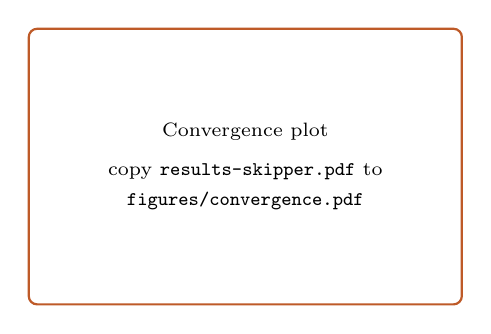
\begin{tikzpicture}
          \node[box,minimum width=55mm,minimum height=35mm,draw=warm,fill=white]
            {\scriptsize Convergence plot\\[1mm]
             \scriptsize copy \texttt{results-skipper.pdf} to\\
             \scriptsize \texttt{figures/convergence.pdf}};
        \end{tikzpicture}%
      }
    \end{column}
  \end{columns}
\end{frame}

% ===========================================================================
\section{Cost}
% ===========================================================================

\begin{frame}{Cost}
  \begin{columns}[T]
    \begin{column}{0.5\textwidth}
      \small
      \begin{tabular}{lr}
        \toprule
        Claude Opus 5.5 (list price) & per M tokens \\
        \midrule
        input              & \$4.00 \\
        output (incl.\ thinking) & \$20.00 \\
        cached input, read & \$0.20 \\
        \bottomrule
      \end{tabular}

      \vspace{3mm}
      Per campaign (30 calls, 8 Sobol):
      \begin{itemize}\small
        \item 22 decision requests + 1 notebook entry
        \item fixed instructions cached $\rightarrow$ cheap repeats
        \item measured: \fillin{FILL IN from Console}
      \end{itemize}
    \end{column}
    \begin{column}{0.46\textwidth}
      Tracked automatically:
      \begin{itemize}\small
        \item each iteration: tokens, cost, running total
        \item end of run: summary
        \item saved in \texttt{<run>\_claude\_decisions.jsonl} and the result pickle
        \item Console Usage / Cost pages are the billed truth
      \end{itemize}
      \vspace{2mm}
      \begin{block}{Perspective}
        \scriptsize
        API cost per campaign is small compared to lab time per image;
        every image the optimizer saves is worth far more.
      \end{block}
    \end{column}
  \end{columns}
\end{frame}

% ===========================================================================
\section{Lab notebook}
% ===========================================================================

\begin{frame}[fragile]{Lab notebook: memory across campaigns}
  \begin{columns}[T]
    \begin{column}{0.46\textwidth}
      \small
      \begin{itemize}
        \item Each API call starts from scratch: no learning between runs
        \item \textbf{End of campaign}: Claude writes a short entry
              (best region, broken settings, sensitivities, suggestions)
        \item \textbf{Start of next campaign}: notebook loaded into Claude's
              instructions as \emph{prior knowledge}
        \item Current measurements take priority over old entries
        \item Plain Markdown file: operators read, edit, add their own notes
      \end{itemize}
    \end{column}
    \begin{column}{0.52\textwidth}
\begin{lstlisting}
# Claude lab notebook

## 2026-10-01 21:40 | module skipper |
   30 measurements (22 new) |
   best F = 0.0296 at Vdd=..., Vr=...

- Best region: ...
- Broken: Vdd above ~ -11 V
  (negative gain, sigma_os > 30000 ADU)
- Most sensitive to: ...
- Next time: ...
\end{lstlisting}
      {\scriptsize Header written by the code (facts); text by Claude.
       Illustrative entry.}
    \end{column}
  \end{columns}
\end{frame}

% ===========================================================================
\section{Comparison and outlook}
% ===========================================================================

\begin{frame}{Gaussian process vs.\ Claude}
  \small
  \begin{tabular}{p{0.24\textwidth}p{0.33\textwidth}p{0.33\textwidth}}
    \toprule
    & Gaussian process & Claude \\
    \midrule
    Information used & parameters and $F$ only & parameters, $F$, image statistics, notes, notebook \\
    Reproducible & yes (fixed seed) & no (choices can vary) \\
    Explains choices & no & yes (thinking summary per point) \\
    Uncertainty model & explicit (GP posterior) & implicit \\
    Memory across runs & warm restart (data only) & data + written lessons \\
    Cost & free & small API cost per campaign \\
    Failure modes & mis-fit on outliers & API availability, safety filters \\
    \bottomrule
  \end{tabular}

  \vspace{3mm}
  Same agents, same outputs: switching is one line in the config.
\end{frame}

\begin{frame}{Open questions and next steps}
  \begin{itemize}
    \item \textbf{Noise of $F$}: repeat one point $\sim$10 times; needed for any
          convergence or ``which point is better'' statement
    \item \textbf{Stopping rule}: today a fixed budget of \texttt{n\_calls};
          options: no-improvement rule, or Claude declares convergence
    \item \textbf{Head-to-head}: GP vs.\ Claude, same day, same budget
    \item \textbf{Better objective}: ask Claude (with literature search) to
          define \emph{``best flat field for astronomy''} as computable criteria,
          reviewed by us, then computed deterministically
          \begin{itemize}\scriptsize
            \item may need flat pairs / several exposure levels per iteration
          \end{itemize}
    \item \textbf{Robustness}: API key check at start-up, flag broken images
          (negative gain), cheaper models (Haiku)
  \end{itemize}
\end{frame}

\begin{frame}{Summary}
  \begin{enumerate}
    \item Reviewed the existing Bayesian optimization of the Skipper-CCD
    \item Rebuilt it as three agents (acquisition, objective, optimizer),
          with results verified identical to the original
    \item Added Claude as a drop-in optimizer that uses the image statistics
          and explains every choice
    \item Made it lab-robust: absolute paths, retries, per-image checkpoints
    \item Added cost tracking and a lab notebook that carries lessons from
          one campaign to the next
  \end{enumerate}
  \vspace{4mm}
  \centering
  {\small Code: \texttt{optimize\_agents.py}, \texttt{agents/}, \texttt{tests/}}
\end{frame}

\end{document}
